\documentclass{uebblatt}

\usepackage{draftwatermark}                                                                       
\definecolor{pink}{rgb}{0.95,0.9,0.95}                                                            
\SetWatermarkText{\textsf{\textcolor{pink}{ENTWURF}}}                                             
\SetWatermarkScale{1}                                                                             

\begin{document}

\maketitle{6}{}

\begin{aufgabe}{Morphismen zwischen fasernden Approximationen}
Seien~$X$ und~$X'$ Objekte einer Modellkategorie. Wähle fasernde
Approximationen~$r : X \to RX$ und~$r' : X' \to RX'$. Seien~$f$ und~$g$
Morphismen~$X \to X'$. Zeige: Wenn~$r' \circ f$ und~$r' \circ g$ zueinander
rechtshomotop sind, so sind auch die induzierten Morphismen~$Rf, Rg : RX \to
RX'$ zueinander rechtshomotop.
\end{aufgabe}

\begin{aufgabe}{Ein Kriterium für Identifizierung rechtshomotoper Morphismen}
Sei~$\M$ eine Modellkategorie und~$\C$ eine beliebige Kategorie. Sei~$F : \M_c
\to \C$ ein Funktor, der auf der vollen Unterkategorie der kofasernden Objekte
definiert ist und azyklische Kofaserungen auf Isomorphismen schickt.
Zeige, dass~$F$ rechtshomotope Morphismen identifiziert.
\end{aufgabe}

\begin{aufgabe}{Eigenschaften von Scheiben- und Koscheibenkategorien}
Sei~$M$ eine Modellkategorie. Sei~$A$ ein Objekt von~$M$. Zeige:
\begin{enumerate}
\item Ist~$M$ links-eigentlich, so auch~$M/A$.
\item Ist~$M$ kofasernd erzeugt, so auch~$M/A$.
\item Ist~$M$ kompakt erzeugt, so auch~$M/A$.
\end{enumerate}
\end{aufgabe}

\vfill
\centering
\href{http://spikedmath.com/182.html}{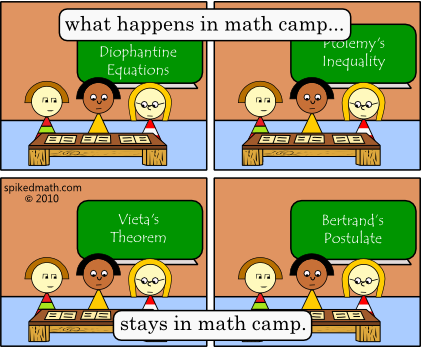
\includegraphics[height=6cm]{images/what-happens-in-math-camp}}
\quad
\href{http://smbc-comics.com/index.php?id=1777}{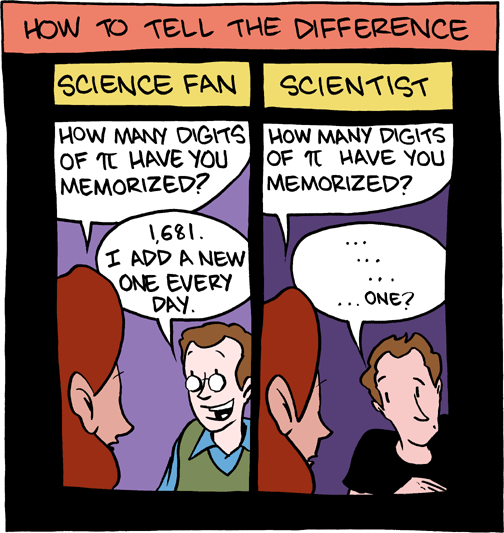
\includegraphics[height=6cm]{images/memorizing-pi}}
\par

\end{document}
